%%\documentclass[aip,jcp]{revtex4-1}
\documentclass[aip
, pra
, showpacs
, aps
, twocolumn
%, onecolumn
, groupedaddress
, floatfix
%, preprint
]{revtex4}
%]{revtex4-1}
\usepackage{graphicx, amsbsy, bm, dcolumn, amsmath}

\newcommand{\etal}{{\em et~al.\/}}
\newcommand{\beq}{\begin{equation}}
\newcommand{\eeq}{\end{equation}}
\newcommand{\barr}{\begin{array}}
\newcommand{\earr}{\end{array}}
\newcommand{\vecr}{{\bf r}}
\newcommand{\dd}{\mbox{d}}
\newcommand{\dr}{\mbox{d} r}
\newcommand{\vare}{\varepsilon}
\newcommand{\calN}{{\cal N}}
\newcommand{\di}{_{\mbox{\tiny{di}}}}
\newcommand{\ex}{_{\mbox{\tiny{ex}}}}



\newcommand{\isum}%
{\mathop{\hbox{$\displaystyle\sum\kern-13.2pt\int\kern1.5pt$}}}

\begin{document}

\title {$J$-matrix calculation of electron-helium $S$-wave scattering. II. Beyond the frozen-core model}

\author{Dmitry A. Konovalov}
\affiliation{ARC Centre for Antimatter-Matter Studies}
\affiliation{Discipline of Information Technology, School of Business, James Cook University, Townsville, Queensland 4811, Australia}

\author{Dmitry V. Fursa}
\affiliation{ARC Centre for Antimatter-Matter Studies,
Curtin University, GPO Box U1987, Perth, Western Australia 6845, Australia}

\author{Igor Bray}
\affiliation{ARC Centre for Antimatter-Matter Studies,
Curtin University, GPO Box U1987, Perth, Western Australia 6845, Australia}



\date{\today}

\begin{abstract}

In the preceding $J$-matrix (JM) paper [D. A. Konovalov {\em et. al.} Phys. Rev. A {\bf 84}, 032707 (2011)],
the $S$-wave $e$-He scattering ($S$-$e$-He) problem was solved within the frozen-core (FC) model of helium for impact energies in the range 0.1-1000eV.
In this sequel, both target electrons are described within the configuration-interaction model of helium obtaining  more accurate (compared to the FC model)
first seven bound states of the $S$-wave helium.
The presented JM calculations solve the $S$-$e$-He problem essentially exactly
for the total elastic, $2^{1,3}S$, $3^{1,3}S$ excitation cross sections below the ionization threshold.
The JM results are confirmed by the corresponding convergent-close-coupling (CCC) calculations creating a challenging benchmark
for any current or future {\it ab initio} electron-atom scattering methods.

Above the ionization threshold, only the elastic and triplet $2^3S$ excitation cross sections are obtained at the benchmark accuracy level.
The total ionization and the rest of excitation cross sections still exhibit noticeable pseudo-resonances (up to 10\% fluctuations),
which could not be eliminated with the considered number of target states (up to 95 eigenstates of He were considered).


\end{abstract}

\pacs{34.80.Dp} %34.80.Dp	Atomic excitation and ionization
\maketitle



\section{INTRODUCTION}


This study focuses on the $S$-wave $e$-He ($S$-$e$-He) scattering,
where the target helium atom is in its ground state before the electron impact,
and where only the partial wave with zero angular momentum ($l=0$) is retained in all calculations
and partial-wave expansions.
The $S$-wave models have proven to be a very productive testing ground for {\it ab initio} scattering theories,
see \cite{T62,HY74p1209,P78,P80,P81,CO84,BS92p53,BST93,KM94pL407,IDHF95,PS96,JS02,JS00l,BRIM99,S99l,MHR02,BS04,Frapiccini10} for the $S$-wave $e$-H scattering ($S$-$e$-H)
and \cite{DHIF94,PMR99,PBFS02,PNBFS04,HMR05R,HMR05,BS10p022715,BS10p022716,KFB11} for  the $S$-$e$-He problem.
The main attraction of the $S$-wave models is that they retain most of the physics complexities of the full
scattering problems while reduce the problems computationally.
In particular, it is somewhat expected and implied that if a theoretical method solves a $S$-wave model, then
the remaining partial waves could be solved with additional computational resources,
which is indeed the case for the convergent-close-coupling (CCC) \cite{FB95},
$R$-matrix (RM) \cite{FLRS94b, SMC2006} and $J$-matrix (JM) \cite{KM94pL741,KM95pL139} methods.


The main goal of this study is to provide high accuracy total elastic and excitation $S$-$e$-He cross sections for 5-100eV impact energies highlighting resonant features of the cross sections.
The need for such benchmark theoretical data is evident from the existing {\em ab initio} attempts to solve the $S$-$e$-He problem.
Reviewing in reverse chronological order, in 2010, \citet{BS10p022715} developed a four-body propagating exterior scaling (PECS) method and reported results claiming to achieve "benchmark" level of accuracy.
However none of their cross sections, including elastic and $2^{1,3}S$ excitation cross sections, displayed any resonances at the accuracy level achieved for the $S$-$e$-H problem \cite{P78}.
In 2005, \citet{HMR05} reported results using
time-dependent exterior complex scaling (TD-ECS), which also failed to described resonance behavior of the cross sections.
In 2002 and 2004, the CCC method \cite{PBFS02,PNBFS04} also did not examine the resonance regions with sufficiently fine energy grid.
This is now corrected to some extent when in 2011 \citet{KFB11} reported the CCC and JM {\em frozen-core}
(FC) results clearly showing the resonances in the elastic and $n=2$ ($2^1S$ and $2^3S$) excitation cross sections.
And finally, the RM method \cite{FLRS94b, SMC2006} has never reported its results for the $S$-$e$-He problem.


The stated goal is attempted and achieved in many aspects by combining advantages of the CCC and JM methods,
where the later has been recently revised \cite{KFB11} by merging it with the Fano's multi-configuration interaction matrix elements \cite{Fano65}.
The CCC method is able to solve the scattering problem very accurately via the Lippmann-Schwinger equation \cite{BS92p6995}.
However, it is not practical to run the CCC method for each of the many thousands of impact energy points required for the final benchmark results.
On the other hand, the JM method is very efficient \cite{HY74p1201,BR76p1491} in calculating a vast number of energy points
but numerical-convergence properties of the JM method remains largely unknown.
The JM and CCC methods are implemented independently and use completely different approaches to solve the scattering equations.
Therefore, the CCC and JM methods can be and were used to cross-verify that their results are convergent within their own numerical parameters at key energy points.

The presented JM method is implemented using Java programming language, which is freely available for MS Windows,
Mac OS, and many versions of Linux or Unix. See \cite{JMatrixWebsite} for information on availability of the results and source code.


\begin{figure*}[htb]
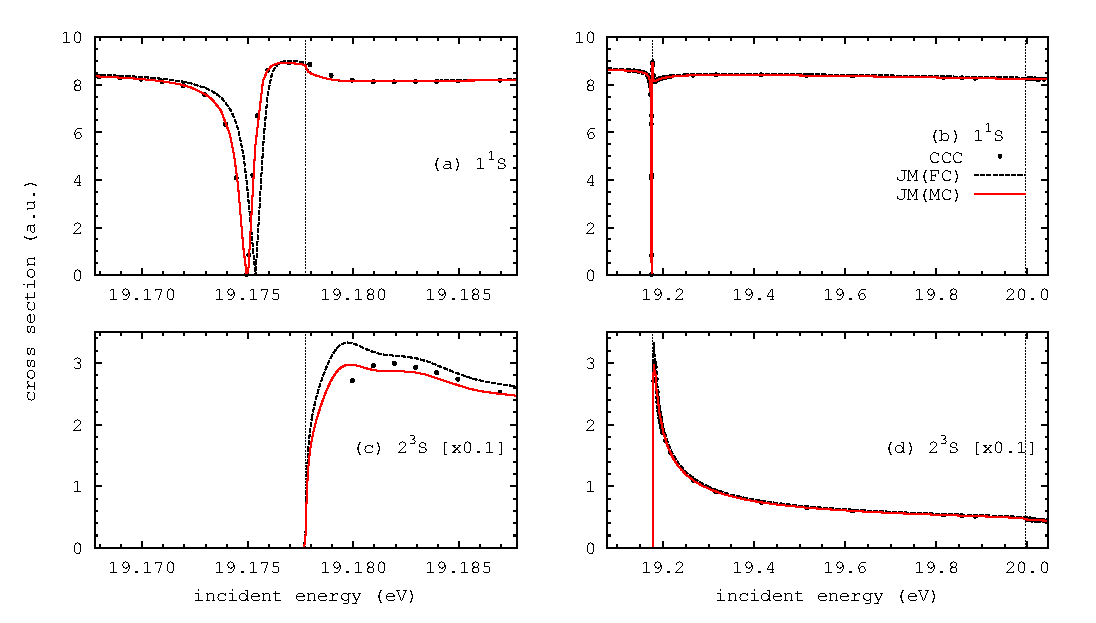
\includegraphics[scale=1]{fig1.ps}
\caption{(Color online) Elastic ($1^1S$),
$n=2$ ($2^3S$ and $2^1S$) and $n=3$ ($3^3S$ and $3^1S$) single-excitation cross sections  below the ionization threshold (23.92eV, Table~\ref{Tab_ENGS}) for the $e$-He $S$-wave scattering model.
Sub-figure (b) zooms in on the $2^3S$ excitation threshold (19.178eV, Table~\ref{Tab_ENGS}) shown by the vertical dashed line.
FC (Frozen-core, $N_c=1$, $N_t=30$), JM ($N_c=7$, $N_t=30$) and CCC ($N_c=3$, $N_t=30$) results  were shifted by 0.17747eV, 0.0018eV and 0.0018eV (Table~\ref{Tab_ENGS}), respectively.
}
\label{Fig_1}
\end{figure*}



\begin{figure}[htb]
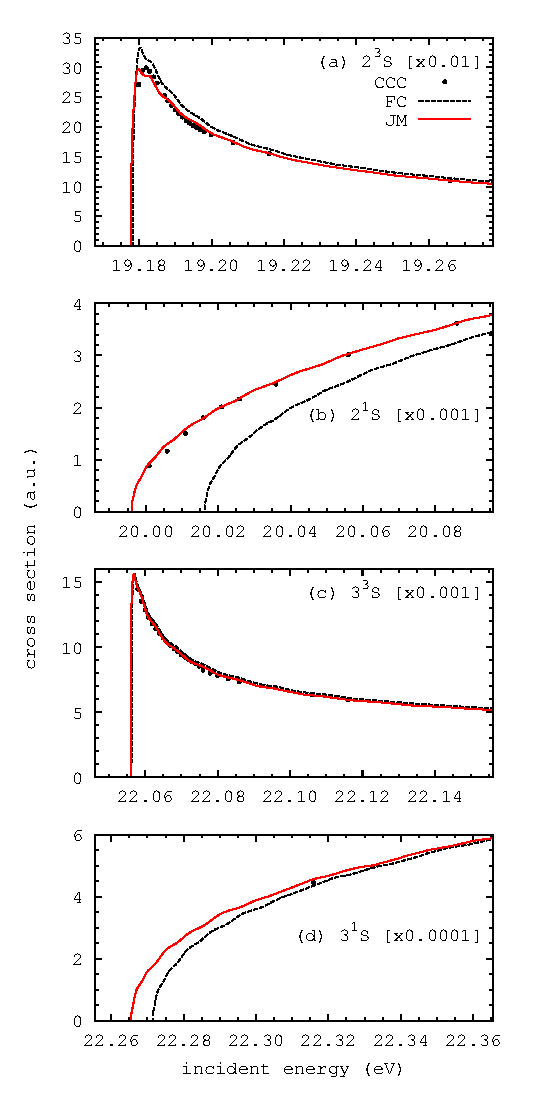
\includegraphics[scale=1]{fig2.ps}
\caption{(Color online)
The same as in Fig.~\ref{Fig_1} but zooming in on the corresponding excitation threshold energies (Table~\ref{Tab_ENGS}).
}
\label{Fig_2}
\end{figure}

\begin{figure}[htb]
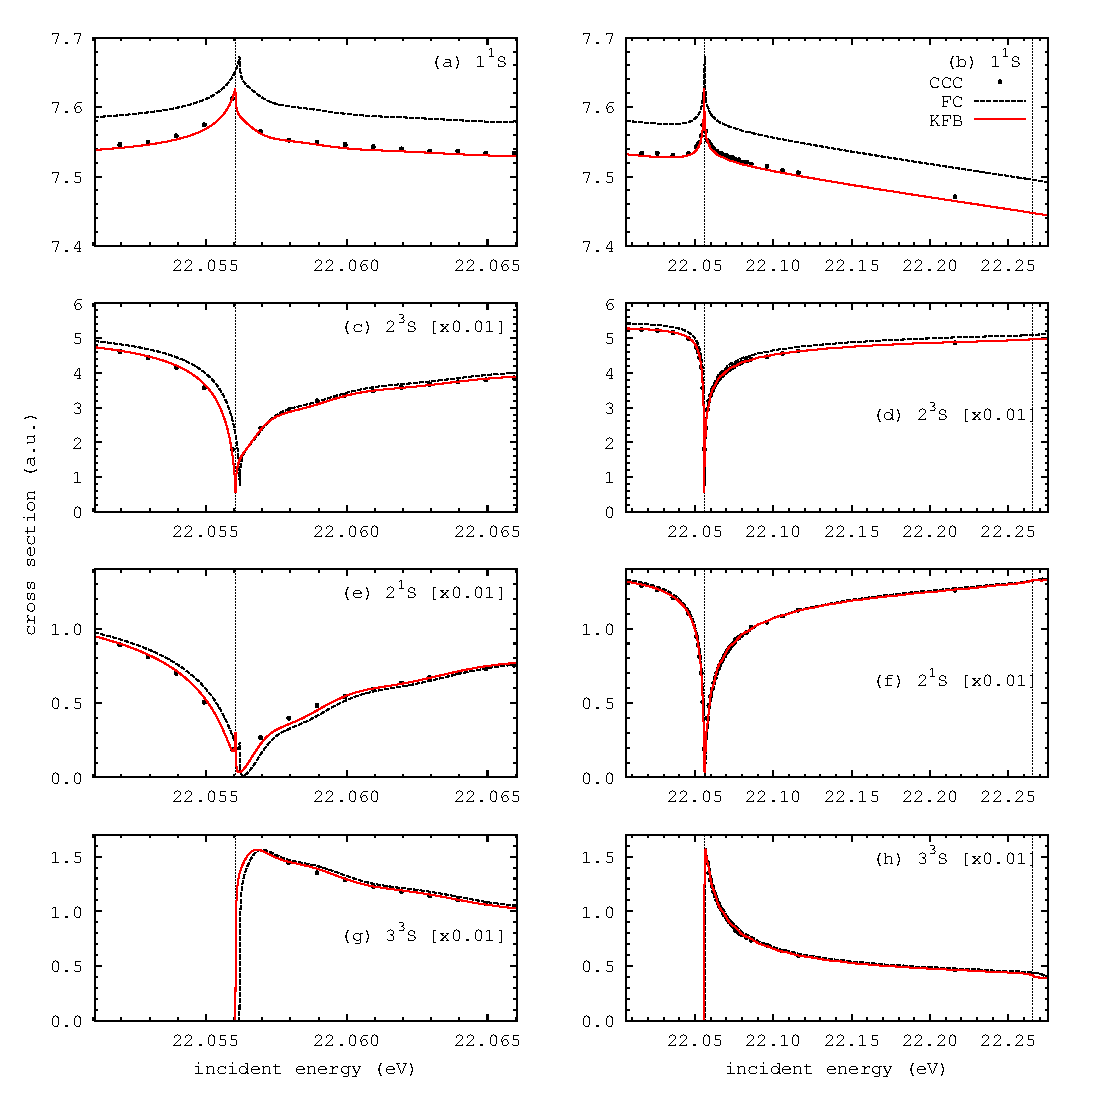
\includegraphics[scale=1]{fig3.ps}
\caption{(Color online)
The same as in Fig.~\ref{Fig_1} but starting from the $3^3S$ threshold
and aligned by incident energies. The $3^1S$, $4^{3,1}S$, ..., $7^{3,1}S$, excitation thresholds (Table~\ref{Tab_ENGS})
are shown by vertical dashed lines (from left to right).
}
\label{Fig_3}
\end{figure}


\begin{figure*}[htb]
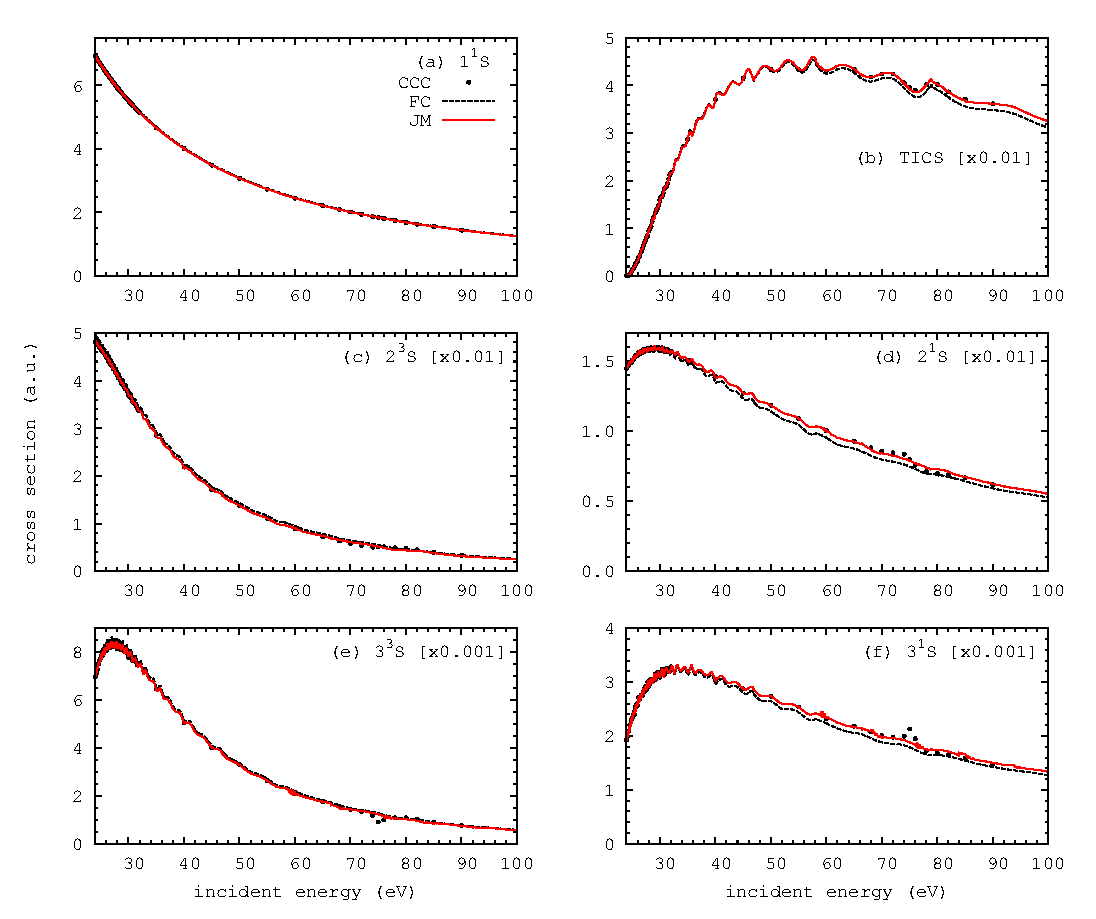
\includegraphics[scale=1]{fig1b.ps}
\caption{(Color online)
The same as in Fig.~\ref{Fig_1} but above the ionization threshold.
}
\label{Fig_1b}
\end{figure*}


\begin{table}[htb]
\caption{\label{Tab_ENGS}
Energy levels [a.u.] and excitation thresholds [eV] of the first nine bound states of helium in the 
$S$-wave model.
$\lambda_c=4$, $\lambda_t=1$, a.u.$=27.2116$eV
}
\begin{ruledtabular}
%\begin{tabular}{lcr}
\begin{tabular}{rlll}
Classification & threshold [eV] & Eigenvalues [a.u] & ($N_c$,$N_t$)   \\
\hline
$\mbox{He}(1s^2,^1S)$ & 0  & -2.879 028 569 1 &  (50,50)   \\ %
            error =          & 0.001 80 & -2.878 962 303   &  (7,30)    \\
            error =          & 0.177 47 & -2.872 506 673   &  (1,30)    \\
\hline
$\mbox{He}(1s2s,^3S)$      & 19.178 & -2.174 264 856 3 & (50,50) \\  %-2.174 264 856 288154 -2.174264856287701, -2.0684901366080752,
                           &    & -2.174 264 618   &  (7,30)   \\
                           &    & -2.174 245 504   &  (1,30)    \\
\hline
$\mbox{He}(1s2s,^1S)$     &  19.996 & -2.144 197 258 7 &  (50,50) \\ %-2.144 197 258 7 31818,
                          &  & -2.144 191 393   &  (7,30)   \\
                          &   & -2.143 449 321   &  (1,30)    \\
\hline
$\mbox{He}(1s3s,^3S)$     & 22.056  & -2.068 490 070   &  (7,30)   \\
                          &        & -2.068 484 660   &  (1,30)    \\
\hline
$\mbox{He}(1s3s,^1S)$     & 22.266   & -2.060 792 356   & (7,30)    \\
                          &          & -2.060 573 161   &  (1,30)    \\
\hline
$\mbox{He}(1s4s,^3S)$    & 22.928  & -2.036 438 560   &  (7,30)    \\
                         &         & -2.036 436 372   &  (1,30)   \\
\hline
$\mbox{He}(1s4s,^1S)$   &  23.011 & -2.033 392 203 &  (7,30)   \\
                        &         & -2.033 300 706 &  (1,30)   \\
\hline
$\mbox{He}(1s5s,^3S)$   &   23.305  & -2.022 583 695   &  (7,30)    \\
                        &           & -2.022 582 608   &  (1,30)    \\
\hline
$\mbox{He}(1s5s,^1S)$   &  23.346   & -2.021 079 423   &  (7,30)    \\
                        &              & -2.021 033 007   &  (1,30)    \\
\hline
$\mbox{He}^+(1s)$       &  23.920 & -2 	 &    Ionization \\

%nc50 -2.8790285691204813, -2.144197258731818, -2.060794037546691, -2.0333785522995016, -2.019784513192403,
%-2.174264856288154, -2.0684901366081845, -2.0364341783161515, -2.021798838036517,

%nc10   -2.878976298682523, -2.1441926558786752, -2.0607927208274255, -2.0333923539473497,
% -2.1742647128049755, -2.0684900966824507, -2.036438571423033,

%nc7 -2.8789623026211353, -2.1441913928180427, -2.0607923564616435, -2.0333922030334937, -2.0210794228323463,
% -2.1742646178307643, -2.068490069685457, -2.036438559573639, -2.022583694613397,

%nc1 -2.872506672905663, -2.143449321021511, -2.06057316103011, -2.033300705504141, -2.0210330065059448,
% -2.1742455043163393, -2.0684846598208337, -2.0364363721136964, -2.022582608219962,

\end{tabular}
\end{ruledtabular}
\end{table}



\section{THEORY}

The JM method \cite{HY74p1201,BR76p1491} is a very general method for solving wide range of scattering problems.
In this study, we continue to develop the version of the JM method that
was previously applied to the $S$-$e$-H \cite{KB10p022708}  and $S$-$e$-He \cite{KFB11} scattering problems.
Hereafter this version will be referred to as the KFB method to assist when discussing its features which are not part of the generic JM method.

When the KFB method was applied to the FC model of helium \cite{KFB11} (one electron was always in the $1s$ state of He$^+$),
the following three sets of functions were used: target basis, JM functions, and Laguerre basis.

{\em Target basis} is a set of $N_t$ orthonormal radial functions $\{P_n(r)\}_{n=1}^{N_t}$,
where $P_n(r)$ is used as the radial component of the $n$'th subshell wave function
when building one- or many-electron wave functions as per the Fano's procedure \cite{Fano65, KFB11}.

{\em JM functions} are the nonorthogonal Laguerre functions $\{\xi_p(r)\}_{p=0}^\infty$ from the original JM method \cite{HY74p1201,BR76p1491},
\beq
\xi_p(r) = x^{l+1} \mbox{e}^{-x /2}
L_p^{2l+1}(x), \ \ \ p = 0, 1, ..., \infty,
\eeq
where $x=\lambda r$, $\lambda$ is Laguerre exponential falloff,
$l \equiv 0$ (for the $S$-model), and $L_p^{\alpha}(x)$ are the associated Laguerre polynomials \cite{abramowitz}.


{\em Laguerre basis} is the set of orthonormal Laguerre functions $\{R_p(r)\}_{p=0}^\infty$,
\beq
R_p(r) = C_p x^{l+1} \mbox{e}^{-x /2}
L_p^{2l+2}(x), \ \ \ p = 0, 1, ..., \infty,
\eeq
\beq
\int_0^\infty dr \ R_p(r) R_{p'}(r) = \delta_{pp'}, \ C_p= \sqrt{\frac{\lambda p!}{ (p+2l+2)!}}.
\eeq
Note that for any fixed $N_t$, both $\{\xi_p(r)\}_{p=0}^{N_t}$ and $\{R_p(r)\}_{p=0}^{N_t}$
span identical functional space \cite{KB10p022708}.


The target basis $\{P_n(r)\}_{n=1}^{N_t}$ is selected or built by diagonalizing a suitable one-electron Hamiltonian \cite{KB10p022708, KFB11}. Then,
the two-electron target-helium wave functions are constructed by allowing first and second helium electrons to occupy the first $N_c$ and $N_t$ radial functions, respectively,
where $N_c$ controls the number of allowed {\em core} excitations with $N_c=1$ being the frozen-core model.


After many numerical experiments, it became apparent that the core excitation functions $\{P_n(r)\}_{n=1}^{N_c}$ should be constructed differently from the rest of the target basis
$\{P_n(r)\}_{n=N_c+1}^{N_t}$. Otherwise, the convergence by $N_c$ is just too slow to be computationally practical.
This is due to the two very different radial scales present in this study.
The short-range core excitations are essentially adjustments to the $1s$-orbital of He$^+$.
While the helium excitations below the ionization threshold resemble $ns$-orbitals of hydrogen and therefore are long-range.
This problem is solved here by using a mix of the short range $\{R^c_p(r)\}_{p=0}^{N_c-1}$ with $\lambda_c=4$
and long-range $\{R^t_p(r)\}_{p=N_c}^{N_t-1}$ with $\lambda_t=1$  basis sets
when constructing the target basis as follows.


The JM method splits the one-electron radial functional space into {\em inner} $\{\xi_p\}_{p=0}^{N-1}$
and {\em outer} $\{\xi_p\}_{p=N}^\infty$
subsets controlled by the number $N$ of JM functions in the inner subset \cite{HY74p1201,BR76p1491}.
In the KFB method, the target basis $\{P_n(r)\}_{n=1}^{N_t}$ must be orthogonal to the outer JM functions $\{\xi_p\}_{p=N}^\infty$, where $N_t<N$.
Let $\lambda \equiv \lambda_t$ and $\hat{I}_t$ be a projection operator into the functional space of $\{R^t_p(r)\}_{p=0}^{N_t-1}$
\beq
\hat{I}_t = \sum_{p=0}^{N_t-1} | R_p^t \rangle \langle R_p^t |,
\eeq
then by construction every function from $\{R^t_p(r)\}_{p=0}^{N_t-1}$ and  $\{R^{ct}_p(r)\}_{p=0}^{N_c-1}$
\beq
R^{ct}_p = \hat{I}_t R^{c}_p, 
\eeq
is orthogonal the outer JM functions. 
Then the final target basis $\{P_n(r)\}_{n=1}^{N_t}$ is constructed by making a single orthonormal basis from 
$\{R^{ct}_p(r)\}_{p=0}^{N_c-1}$ and $\{R^t_p(r)\}_{p=N_c}^{N_t-1}$
via the Gram-Schmidt process.


Note that in the CCC method the final target basis 
$\{P^{\mbox{{\tiny 3C}}}_n(r)\}_{n=1}^{N_t}$ is also built via the Gram-Schmidt process but from
$\{R^{c}_p(r)\}_{p=0}^{N_c-1}$ and $\{R^t_p(r)\}_{p=N_c}^{N_t-1}$ sets, that is, the $R^{ct}_p$ functions were not required.
 



\section{RESULTS}

See Supplemental Material at [URL will be inserted by publisher] for the results in tabular form.

The number $N$ is the key JM parameter responsible for the convergence of any implementation of the JM method.
That is, the larger the $N$, the more accurate the corresponding JM results are expected to be.
Within the current KFB method, maximum value of $N$ is limited to around 100 so that the method remains to be easily accessible
to wider research community. All presented in this study KFB results were still calculated on a consumer-grade laptop.


The following KFB computational parameters were used, see \cite{KB10p022708} for explanation of the parameters:
$\lambda_c=4$, $\lambda_t=1$, $N_t=30$, $N=100$, $\ln(c)=-5 - 2\ln(Z_{\mbox{\tiny{He}}} )$, $Z_{\mbox{\tiny{He}}}=2$, $r_{\max}=500$,
$M_{LCR}=2001$, where the radial grid was between zero and $r_{\max}$ and
$M_{LCR}$ is the number of equally spaced points in the radial LCR grid \cite{KB10p022708}.
Hereafter FC, JM and CCC denote results obtained with $N_c=1$, $N_c=7$ and $N_c=3$, respectively. 
When converting to eV scale, 27.2116 eV was used as the atomic unit of energy (or Hartree).

Table~\ref{Tab_ENGS} shows first nine eigenvalues from diagonalizations of $S$-wave helium Hamiltonian. 
Selecting $\lambda_c=4$ creates the first target radial function $P_1(r)$ numerically identical to the exact $1s$ state of He$^+$, 
when $N_t$ is sufficiently large as is the case for the used $N_t=30$.
The main improvement of the $N_c=7$ basis over the froze-core case ($N_c=1$) is in the ground state of helium, where 
the first seven significant figures \cite{G94} were obtained by using  $\{R^{c}_p(r)\}_{p=0}^{N_c-1}$ as the basis for both electrons with $N_c=50$ and $\lambda_c=4$.

Fig.~\ref{Fig_1} shows that if the FC results are shifted by the FC ground energy error (0.17747eV, see Table~\ref{Tab_ENGS}), 
the FC and JM results become very close. This means that most of the scattering dynamics  is essentially due to 
the movement of one electron in the field of $1s$ state of He$^+$. Fig.~\ref{Fig_1}(b)





\section{CONCLUSIONS}





\begin{acknowledgments}
This work was supported by the Australian Research Council. IB
acknowledges the Australian National Computational Infrastructure
Facility and its Western Australian node iVEC.
\end{acknowledgments}



\bibliographystyle{apsrev}
\bibliography{../bibtex/qm_references}

\end{document}
